\chapter{基于自回归流式解码的高质量语音交互大模型}\label{chap:llama-omni2}

\section{引言}

上一章提出的LLaMA-Omni通过基于CTC的非自回归语音解码器实现了文本与语音响应的同步流式生成，响应延迟低至236毫秒。然而，非自回归建模方式在语音生成能力上存在固有局限：CTC解码器独立预测每个位置的离散语音单元，难以建模单元之间的长程依赖关系，导致生成语音的自然度和表现力不足。此外，LLaMA-Omni的语音输出仅限于单一的标准音色，无法满足实际应用中对多样化语音风格的需求。如何在保持低延迟流式交互的同时大幅提升语音生成的质量和自然度，是语音交互模型走向实用化的关键问题。

当前，端到端语音-语言模型的构建主要有两条技术路线。一类是原生语音-语言模型（Native SpeechLM），将语音离散化为词元，在统一的语言模型中联合建模语音和文本\citep{zhang-etal-2023-speechgpt, glm4voice, kyutai2024moshi}。这类方法可以利用大规模无监督语音数据进行预训练，有望产生更接近人类的语音表现力。然而，原生方法通常需要百万小时级别的语音数据进行预训练，训练成本极高，且大规模语音预训练可能导致模型原有的文本能力出现灾难性遗忘。另一类是模块化语音-语言模型（Modular SpeechLM），在大语言模型前后分别添加语音编码器和语音解码器来处理语音的理解和生成\citep{fang2025llamaomni, xiong2024freeze}。模块化方法的优势在于能够充分利用各组件的已有能力，仅需少量微调即可使模型具备语音交互能力，同时保留大语言模型原有的文本理解和生成能力。然而，现有模块化方法中的语音解码器多采用非自回归建模，生成语音的自然度仍不理想。

针对上述问题，本章的核心研究目标是：设计一种自回归流式语音解码器，使其既能建模语音词元之间的序列依赖关系以提升生成质量，又能在大语言模型生成文本的过程中同步流式地产生语音响应以保持低延迟。

为此，本章提出了LLaMA-Omni 2，一系列参数规模从0.5B到14B的模块化语音交互模型。LLaMA-Omni 2采用Qwen2.5系列模型\citep{qwen2.5}作为基础大语言模型，使用Whisper\citep{whisper}编码器作为语音编码器。在语音解码方面，本章借鉴CosyVoice 2\citep{du2024cosyvoice}的流式语音合成方案，设计了由TTS语言模型、因果流匹配模型和HiFi-GAN声码器组成的自回归流式语音生成管线。其中，TTS语言模型从Qwen2.5-0.5B初始化，通过门控融合机制将大语言模型的隐状态和文本词元嵌入进行自适应融合，并采用读写交替策略实现流式生成。整个模型仅需200000条多轮语音对话数据即可完成训练，无需额外的ASR或TTS数据。

在语音问答和语音指令遵循任务上的实验结果表明，LLaMA-Omni 2在语音到文本和语音到语音两种设置下均超越了LLaMA-Omni和GLM-4-Voice\citep{glm4voice}，同时响应延迟低于600毫秒，满足实时交互的需求。消融实验进一步验证了门控融合机制、TTS预训练策略和读写策略等设计选择的有效性。


\section{方法介绍}

本节介绍LLaMA-Omni 2的模型架构、训练策略和流式推理方法。

\subsection{模型架构}

如图\ref{fig:llamaomni2}所示，LLaMA-Omni 2的核心是一个大语言模型，本章选用Qwen2.5系列模型作为基础模型。下面分别介绍如何为大语言模型添加语音理解和流式语音生成能力。在以下描述中，用$\mathcal{M}_\text{LLM}$表示大语言模型。对于一条指令-响应对，语音指令记为$X$，文本响应和语音响应分别记为$Y^T$和$Y^S$。

\begin{figure}[htbp]
    \centering
    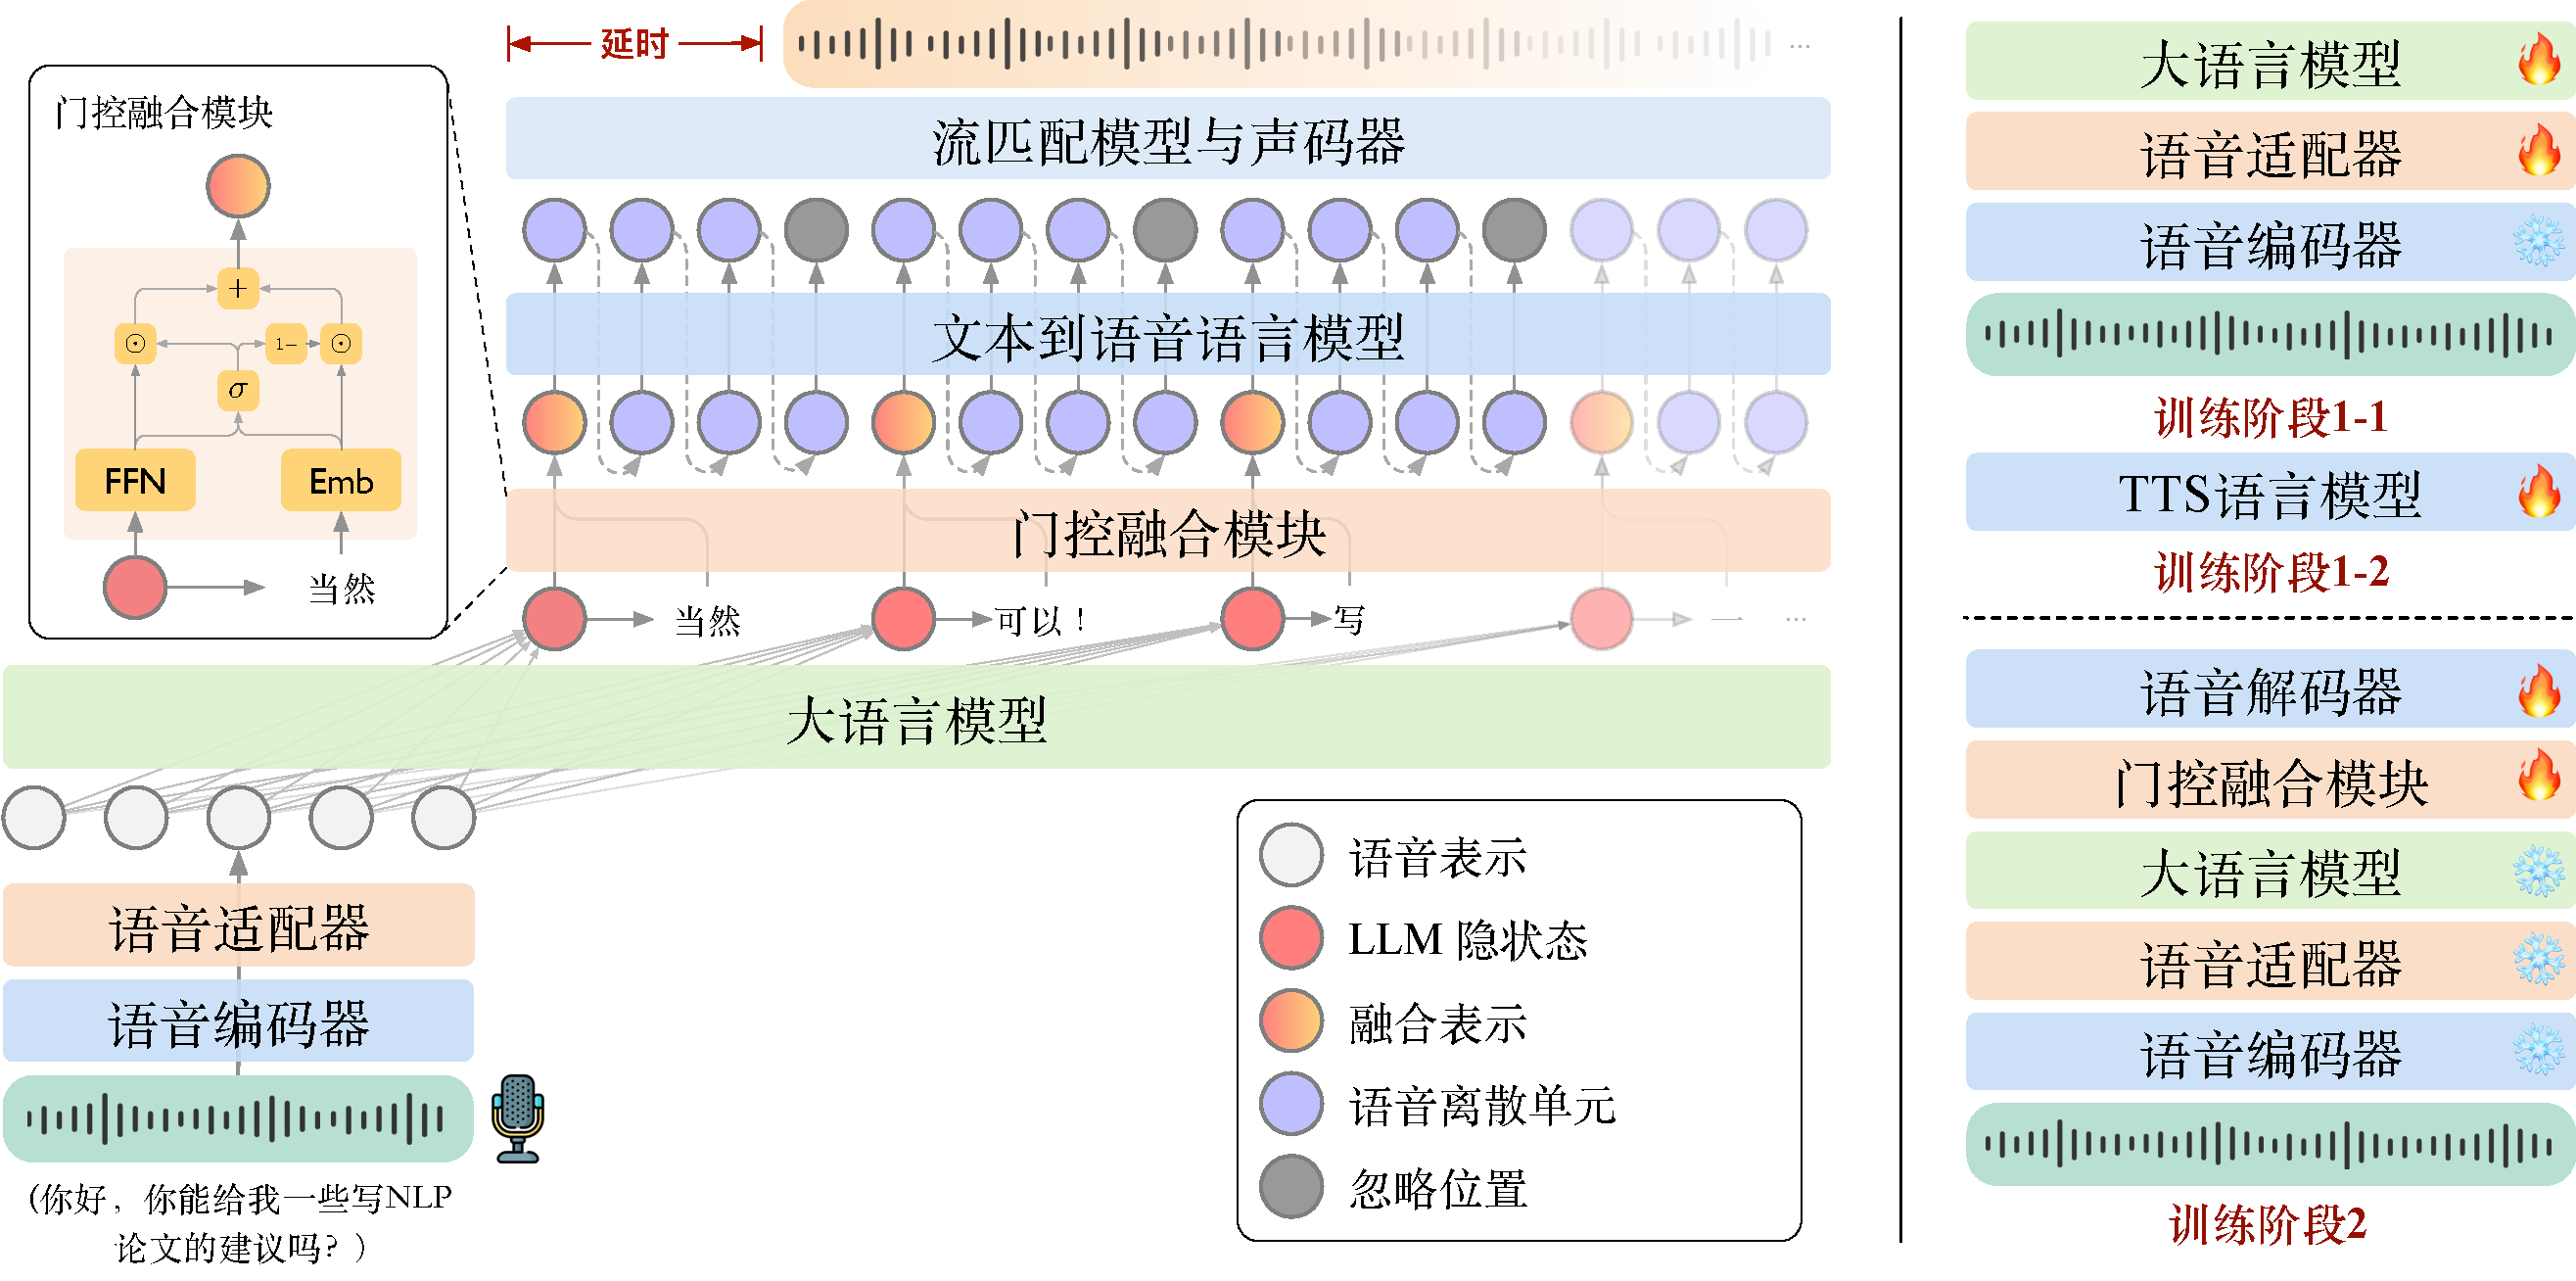
\includegraphics[width=0.95\textwidth]{Img/LLaMA_Omni2.pdf}
    \bicaption{\enspace LLaMA-Omni 2模型架构与训练策略}{\enspace Model architecture and training strategy of LLaMA-Omni 2}
    \label{fig:llamaomni2}
\end{figure}


\textbf{语音理解}\quad 语音理解部分的设计与上一章LLaMA-Omni相同。本章采用Whisper-large-v3\citep{whisper}的编码器作为语音编码器，将输入语音转换为表示序列。编码后的表示经过语音适配器映射到大语言模型的嵌入空间。语音适配器由下采样模块和前馈网络（FFN）组成：下采样模块将每$k$个连续帧沿特征维度拼接，拼接后的表示再通过前馈网络进行编码。最终得到的语音表示输入大语言模型。在整个训练过程中，语音编码器的参数保持冻结。

\textbf{语音分词器}\quad 为了将语音响应$Y^S$转换为离散词元序列，本章采用CosyVoice 2\citep{du2024cosyvoice}中预训练的语音分词器。该分词器通过在SenseVoice-Large\citep{an2024funaudiollm}语音识别模型的编码器中插入有限标量量化（Finite Scalar Quantization, FSQ）\citep{mentzer2024finite}模块实现。FSQ模块将编码器的中间表示投影到低秩空间，并通过取整操作进行离散化。最终，语音响应$Y^S$被转换为词元序列$Y^U = [y^U_1, \ldots, y^U_M]$，帧率为每秒25个词元，每个词元$y^U_i \in \{K \in \mathbb{N} \mid 0 \leq K < 6561\}$。

\textbf{TTS语言模型}\quad 将语音响应转换为离散词元后，本章使用一个仅解码器的Transformer\citep{transformer}来建模从大语言模型输出到语音词元的条件语言模型，记为$\mathcal{M}_\text{TTS}$。该模型从Qwen2.5-0.5B初始化，并将词表扩展为$\mathbb{V}' = \mathbb{V} \cup \{ \langle i \rangle \mid i \in \mathbb{N}, 0 \leq i < 6561 \}$，其中$\mathbb{V}$为原始词表。词表扩展使模型能够生成语音词元。

$\mathcal{M}_\text{TTS}$的输入来自大语言模型的输出，具体包含两个部分：连续隐状态和从隐状态中采样得到的文本词元。前者包含上下文信息，后者提供精确的文本内容。本章同时使用这两部分作为TTS语言模型的输入，使模型在生成语音词元时既能考虑当前上下文，又能确保与文本响应的对齐。训练时大语言模型采用教师强制（Teacher Forcing），其输出隐状态记为$\mathbf{H} = [\mathbf{h}_1, \ldots, \mathbf{h}_N]$，其中$\mathbf{h}_i = \mathcal{M}_\text{LLM}(X, Y^T_{<i})$，对应的文本为真实标签$Y^T = [y^T_1, \ldots, y^T_N]$。本章首先通过一个两层前馈网络将隐状态映射到$\mathcal{M}_\text{TTS}$的嵌入维度，同时获取文本词元的嵌入：
\begin{align}
    \mathbf{e}^{\text{hidden}}_i &= \text{FFN}(\mathbf{h}_i) \\
    \mathbf{e}^{\text{emb}}_i &= \text{Emb}(y^T_i)
\end{align}
其中$\text{Emb}(\cdot)$为$\mathcal{M}_\text{TTS}$的嵌入层。随后，通过逐元素门控融合机制将两种表示进行自适应融合。具体地，门控向量$\mathbf{g}_i$的计算如下：
\begin{equation}
    \mathbf{g}_i = \sigma\left( \mathbf{W}_g \left[ \mathbf{e}_i^{\text{hidden}} \parallel \mathbf{e}_i^{\text{emb}} \right] + \mathbf{b}_g \right)
\end{equation}
其中$\parallel$表示拼接操作，$\sigma$为Sigmoid函数，$\mathbf{W}_g \in \mathbb{R}^{2d \times d}$和$\mathbf{b}_g \in \mathbb{R}^d$分别为门控的权重和偏置参数，$d$为$\mathcal{M}_\text{TTS}$的嵌入维度。融合后的表示计算为：
\begin{equation}
    \mathbf{c}_i = \mathbf{g}_i \odot \mathbf{e}_i^{\text{hidden}} + (1 - \mathbf{g}_i) \odot \mathbf{e}_i^{\text{emb}}
\end{equation}
其中$\odot$表示逐元素乘法。融合后的表示$\mathbf{C} = [\mathbf{c}_1, \ldots, \mathbf{c}_N]$输入$\mathcal{M}_\text{TTS}$用于生成语音词元。

为了实现流式生成，即在大语言模型输出的过程中同步生成语音词元，本章采用类似CosyVoice 2的``读$\mathcal{R}$-写$\mathcal{W}$''策略。具体地，将融合后的表示$\mathbf{C}$与语音词元$Y^U$按照预定义的比例$\mathcal{R}:\mathcal{W}$进行交错排列：每读入$\mathcal{R}$个融合表示，模型生成$\mathcal{W}$个语音词元。当所有融合表示读入完毕后，模型继续生成剩余的语音词元直至结束。训练时仅对生成的语音词元计算交叉熵损失：
\begin{equation}
    \mathcal{L}_\text{TTS} = -\sum_{i=1}^{M} \log P\left(y^U_i \mid \mathbf{C}_{\leq \min\left(\left\lfloor \frac{i-1}{\mathcal{W}}+1 \right\rfloor \cdot \mathcal{R},\, N\right)},\, Y^U_{<i}\right)
\end{equation}
其中$\mathbf{C}_{\leq \min(\lfloor \frac{i-1}{\mathcal{W}}+1 \rfloor \cdot \mathcal{R},\, N)}$表示已读入的融合表示。

\textbf{流匹配模型与声码器}\quad $\mathcal{M}_\text{TTS}$生成的语音词元进一步通过一个因果分块流匹配模型\citep{lipman2023flow}以流式方式合成梅尔谱。每当$\mathcal{M}_\text{TTS}$生成$\mathcal{W}$个语音词元，这些词元即作为一个块送入流匹配模型进行梅尔谱合成。合成的梅尔谱再通过HiFi-GAN\citep{hifigan}声码器生成最终的语音波形。本章直接使用CosyVoice 2中预训练的流匹配模型和声码器。

\subsection{训练策略}

LLaMA-Omni 2的训练仅依赖200000条多轮语音对话数据，不使用任何额外的ASR或TTS数据。训练过程分为两个阶段，如图\ref{fig:llamaomni2}右侧所示。

\textbf{第一阶段}\quad 第一阶段分别训练语音到文本和文本到语音两个方向的能力。训练数据由多轮语音对话数据中提取的语音指令-文本响应对和文本响应-语音响应对组成。对于语音到文本方向（阶段I(a)），冻结语音编码器，训练语音适配器和大语言模型，使用交叉熵损失。对于文本到语音方向（阶段I(b)），训练TTS语言模型，使用交叉熵损失。在此阶段中，门控融合模块不参与训练，$\mathcal{M}_\text{TTS}$仅接收文本词元嵌入作为输入。

\textbf{第二阶段}\quad 第二阶段训练模型的语音到语音生成能力，使用完整的语音对话数据。此阶段冻结语音编码器、语音适配器和大语言模型的所有参数，仅训练门控融合模块和$\mathcal{M}_\text{TTS}$。通过这种分阶段训练策略，TTS语言模型在第一阶段已获得基本的语音合成能力，在第二阶段则进一步学习利用大语言模型的隐状态信息来提升语音生成质量。

\subsection{流式推理}

在推理阶段，大语言模型基于语音指令自回归地生成文本响应。每生成$\mathcal{R}$个文本词元后，其隐状态和对应的文本词元经门控融合模块送入$\mathcal{M}_\text{TTS}$，生成$\mathcal{W}$个语音词元，再经流匹配模型和声码器合成一段语音。这样，文本和语音响应可以同步生成。首个语音片段的响应延迟可分解为：
\begin{equation}
    \mathcal{T}_\text{total} = \mathcal{T}_\text{LLM}(\mathcal{R}) + \mathcal{T}_\text{TTS}(\mathcal{W}) + \mathcal{T}_\text{FM}(\mathcal{W}) + \mathcal{T}_\text{Voc}(2\mathcal{W})
    \label{eq:llamaomni2_latency}
\end{equation}
其中$\mathcal{T}_\text{LLM}(\mathcal{R})$和$\mathcal{T}_\text{TTS}(\mathcal{W})$分别为大语言模型和TTS语言模型生成$\mathcal{R}$和$\mathcal{W}$个词元所需的时间，$\mathcal{T}_\text{FM}(\mathcal{W})$和$\mathcal{T}_\text{Voc}(2\mathcal{W})$分别为流匹配模型和声码器处理$\mathcal{W}$和$2\mathcal{W}$个词元所需的时间。声码器的输入长度为$2\mathcal{W}$，这是因为梅尔谱的帧率为每秒50帧，是语音词元帧率的两倍。


\section{多轮对话数据集构建}

本节介绍多轮语音对话数据的构建过程。训练数据在上一章InstructS2S-200K数据集的基础上进行扩展。InstructS2S-200K包含200000条适用于语音交互场景的单轮指令遵循样本，由Alpaca\citep{alpaca}和UltraChat\citep{ultrachat}数据集经大语言模型改写而成。本章将其扩展为多轮对话格式。

具体地，对于每条样本，首先从泊松分布中采样对话轮数$N \sim \text{Poisson}(\lambda=2)$，并将$N$截断到1至5的范围内。随后，使用Llama-3.3-70B-Instruct\citep{dubey2024llama3}模型迭代生成对话内容：对于第$i$轮对话，基于前$i-1$轮的对话历史生成当前轮的指令和响应。通过这种方式，获得200000条多轮文本对话样本。

接下来需要将文本对话转换为语音。为模拟真实应用场景，指令端采用多样化的声音，而响应端保持统一的声音。对于每条多轮对话，首先使用fish-speech\citep{fish-speech-v1.4}模型以随机声音合成一段短语音作为声纹提示，再使用CosyVoice 2模型在克隆该声纹的条件下将指令合成为语音。这种方式确保了同一对话内不同轮次的指令声音保持一致，同时不同对话之间具有声音多样性。对于所有响应，使用统一的声纹提示通过CosyVoice 2模型合成语音。


\section{实验结果与分析}

\subsection{实验设置}

\subsubsection{模型配置}

语音编码器采用Whisper-large-v3的编码器。语音适配器首先进行5倍下采样，再通过中间维度为2048的前馈网络进行编码。大语言模型选用Qwen2.5系列，包括Qwen2.5-0.5B/1.5B/3B/7B/14B-Instruct五个规模，对应的模型分别称为LLaMA-Omni 2-0.5B/1.5B/3B/7B/14B。TTS语言模型从Qwen2.5-0.5B初始化，读写策略设置为$\mathcal{R}=3$，$\mathcal{W}=10$。语音分词器、流匹配模型和声码器直接取自CosyVoice 2。

\subsubsection{训练细节}

训练数据使用上节构建的200000条多轮语音对话数据，采用两阶段训练。阶段I(a)冻结语音编码器，训练语音适配器和大语言模型的全部参数，批次大小为32，训练3个轮次，峰值学习率为$5 \times 10^{-5}$。阶段I(b)训练TTS语言模型，批次大小为32，训练5个轮次，峰值学习率为$5 \times 10^{-4}$。阶段II冻结语音编码器、语音适配器和大语言模型，训练门控融合模块和TTS语言模型，批次大小为32，训练1个轮次，峰值学习率为$1 \times 10^{-3}$。所有阶段均使用前3\%步数的预热策略和余弦退火学习率调度器。LLaMA-Omni 2-14B在4块NVIDIA H800 GPU上训练，其余模型在4块NVIDIA L40 GPU上训练。

\subsubsection{评价指标}

本章在两个任务上进行评测：语音问答（Spoken Question Answering, SpokenQA）和语音指令遵循。对于两个任务，分别评测模型的语音到文本和语音到语音能力。语音到语音的评测通过Whisper-large-v3将语音响应转录为文本后，再使用与语音到文本相同的评测方法。大语言模型的解码均使用贪心搜索以确保结果稳定，TTS语言模型使用温度为1.0的采样解码。

\textbf{SpokenQA准确率}\quad 语音问答任务向模型提出口语形式的问题，检查参考答案是否出现在模型响应中，计算准确率。本章在Llama Questions\citep{nachmani2024spoken}和Web Questions\citep{berant-etal-2013-semantic}两个基准上进行评测。Web Questions数据集中的问题为文本形式，使用CosyVoice 2合成为语音。

\textbf{ChatGPT分数}\quad 使用GPT-4o\citep{gpt4o}对模型响应进行1到5分的评分，综合考虑帮助性、相关性、流畅性和语音交互适用性等因素。对于语音到语音任务，先使用Whisper-large-v3将语音响应转录为文本再进行评分。

\textbf{ASR-WER}\quad 使用Whisper-large-v3将语音响应转录为文本，计算转录文本与模型生成的文本响应之间的词错误率，衡量文本响应与语音响应之间的一致性。

\textbf{UTMOS}\quad 使用UTMOS\citep{saeki22c_interspeech}模型预测生成语音的自然度主观评分。

\textbf{延迟}\quad 在单块NVIDIA L40 GPU上测量从接收语音指令到生成首个语音片段的时间。

\subsubsection{基线系统}

本章选取以下语音-语言模型作为基线系统：
\begin{itemize}
    \item \textbf{LLaMA-Omni}\citep{fang2025llamaomni}：上一章提出的实时语音交互模型，使用基于CTC的流式语音解码器同步生成文本和语音响应，语音单元块大小设为$\Omega = 40$。
    \item \textbf{GLM-4-Voice}\citep{glm4voice}：一个在百万小时级语音数据上预训练的原生语音-语言模型，通过以固定比例13:26交替生成文本和语音词元实现实时交互。
    \item \textbf{SpeechGPT}\citep{zhang-etal-2023-speechgpt}：一个支持语音输入输出的语音-语言模型，采用模态链提示方式进行解码。
    \item \textbf{TWIST}\citep{hassid2024textually}：一个基于文本预训练的语音-语言模型。
    \item \textbf{Spectron}\citep{nachmani2024spoken}：一个端到端的语音问答模型。
    \item \textbf{Moshi}\citep{kyutai2024moshi}：一个支持实时全双工语音对话的原生语音-语言模型。
\end{itemize}

\subsection{主要结果}

\begin{table}[!htbp]
    \bicaption{\enspace 语音问答和语音指令遵循任务的主要结果}{\enspace Main results on spoken question answering and speech instruction following}
    \label{tab:llamaomni2_main}
    \centering
    \small
    \resizebox{\linewidth}{!}{
    \begin{tabular}{lccccccccc}
        \toprule
        \multirow{3}{*}{\textbf{模型}} & \multicolumn{4}{c}{\textbf{语音问答准确率$\uparrow$}} & \multicolumn{5}{c}{\textbf{语音指令遵循}} \\
        \cmidrule{2-5} \cmidrule{6-10}
        & \multicolumn{2}{c}{\textbf{Llama Questions}} & \multicolumn{2}{c}{\textbf{Web Questions}} & \multicolumn{2}{c}{\textbf{ChatGPT分数$\uparrow$}} & \multirow{2}{*}{\textbf{ASR-WER$\downarrow$}} & \multirow{2}{*}{\textbf{UTMOS$\uparrow$}} & \multirow{2}{*}{\textbf{延迟(ms)$\downarrow$}} \\
        & \textbf{S2T} & \textbf{S2S} & \textbf{S2T} & \textbf{S2S} & \textbf{S2T} & \textbf{S2S} & & & \\
        \midrule
        TWIST & - & 4.0 & - & 1.5 & - & - & - & - & - \\
        SpeechGPT & 21.6 & - & 6.5 & - & 2.98 & 2.17 & 40.01 & 3.51 & 5587.94 \\
        Spectron & 21.9 & - & 6.1 & - & - & - & - & - & - \\
        Moshi (7B) & 62.3 & 21.0 & 26.6 & 9.2 & - & - & - & - & - \\
        GLM-4-Voice (9B) & 64.7 & 50.7 & 32.2 & 15.9 & 4.16 & 4.09 & 9.02 & 3.48 & 1562.81 \\
        LLaMA-Omni (8B) & 67.7 & 49.0 & 33.4 & 23.7 & 3.99 & 3.52 & 5.95 & 3.67 & \textbf{346.73} \\
        \midrule
        LLaMA-Omni 2-0.5B & 45.7 & 38.7 & 17.7 & 16.8 & 3.24 & 3.20 & \textbf{2.64} & 4.21 & 542.71 \\
        LLaMA-Omni 2-1.5B & 62.0 & 52.7 & 28.2 & 26.6 & 4.01 & 3.91 & 3.06 & \textbf{4.22} & 552.76 \\
        LLaMA-Omni 2-3B & 64.3 & 55.7 & 30.5 & 28.0 & 4.24 & 4.14 & 3.37 & \textbf{4.22} & 567.84 \\
        LLaMA-Omni 2-7B & 70.3 & 60.7 & 34.5 & 31.3 & 4.28 & 4.15 & 3.26 & 4.19 & 582.91 \\
        LLaMA-Omni 2-14B & \textbf{73.0} & \textbf{62.7} & \textbf{40.4} & \textbf{37.1} & \textbf{4.56} & \textbf{4.35} & 3.89 & 4.20 & 663.32 \\
        \bottomrule
        \multicolumn{10}{l}{\scriptsize 注：S2T和S2S分别代表语音到文本和语音到语音。所有LLaMA-Omni 2系列模型均采用$\mathcal{R}=3$, $\mathcal{W}=10$的读写策略。}
    \end{tabular}}
\end{table}


表\ref{tab:llamaomni2_main}展示了语音问答和语音指令遵循任务上的主要结果。

在语音问答任务上，对于参数规模相近的模型，LLaMA-Omni 2-7B在语音到文本和语音到语音两种设置下均优于GLM-4-Voice和LLaMA-Omni。LLaMA-Omni 2显著缩小了语音到文本与语音到语音之间的性能差距：在Web Questions基准上，GLM-4-Voice的准确率从32.2降至15.9，下降16.3个百分点；LLaMA-Omni从33.4降至23.7，下降9.7个百分点；而LLaMA-Omni 2-7B仅从34.5降至31.3，下降3.2个百分点，说明自回归语音解码器大幅提升了语音生成能力。对于不同参数规模的模型，准确率随大语言模型规模的增大而提高，表明LLaMA-Omni 2能够有效利用大语言模型的内在能力。较小规模的LLaMA-Omni 2-1.5B/3B在语音到语音设置下已超越GLM-4-Voice和LLaMA-Omni的准确率，适合部署在边缘设备上。LLaMA-Omni 2-14B相比7B模型取得了显著的准确率提升，体现了该方法在扩展到更大模型时的潜力。

在语音指令遵循任务上，LLaMA-Omni 2-3B/7B/14B在语音到文本和语音到语音设置下均优于GLM-4-Voice和LLaMA-Omni。模型性能同样随大语言模型规模的增大而提升，LLaMA-Omni 2-14B取得了最优结果。ASR-WER方面，LLaMA-Omni 2系列模型整体较低，显著低于之前的基线系统，证明了文本与语音响应之间的高一致性。语音质量方面，得益于CosyVoice 2的因果流匹配模型，LLaMA-Omni 2在流式合成条件下取得了较高的UTMOS分数，显著优于基线模型。延迟方面，LLaMA-Omni 2的响应延迟约为600毫秒，虽略高于LLaMA-Omni，但仍满足实时交互的需求，且显著低于GLM-4-Voice。

\subsection{消融实验}

本节在LLaMA-Omni 2-7B模型上进行一系列消融实验，分析不同因素对整体性能的影响。

\subsubsection{门控融合机制}

\begin{table}[!htbp]
    \bicaption{\enspace 门控融合机制的消融实验}{\enspace Ablation study on the gate fusion module}
    \label{tab:llamaomni2_ablation}
    \centering
    \small
    \begin{tabular}{lcc}
        \toprule
        \textbf{模型} & \textbf{ChatGPT分数(S2S)} & \textbf{ASR-WER} \\
        \midrule
        LLaMA-Omni 2-7B & \textbf{4.15} & \textbf{3.26} \\
        \quad 去除门控融合 & 4.02 & 4.89 \\
        \quad\quad 去除文本嵌入 & 3.88 & 6.83 \\
        \bottomrule
    \end{tabular}
\end{table}


表\ref{tab:llamaomni2_ablation}展示了门控融合机制的消融实验结果。门控融合模块使模型能够自适应地融合大语言模型的隐状态和文本词元嵌入，同时利用上下文信息和文本内容。当去除门控融合模块，将两部分表示直接相加（$\mathbf{e}_i^\text{hidden} + \mathbf{e}_i^\text{emb}$）作为TTS语言模型的输入时，ChatGPT分数从4.15下降到4.02，ASR-WER从3.26升高到4.89。进一步去除文本嵌入，仅使用隐状态（$\mathbf{e}_i^\text{hidden}$）作为输入时，性能进一步下降，ChatGPT分数降至3.88，ASR-WER升至6.83。这一结果验证了文本嵌入输入的必要性以及门控融合机制的有效性。

\subsubsection{TTS预训练策略}

\begin{table}[!htbp]
    \bicaption{\enspace TTS预训练策略的消融实验}{\enspace Ablation study on TTS pretraining strategies}
    \label{tab:llamaomni2_pretrain}
    \centering
    \small
    \begin{tabular}{lcc}
        \toprule
        \textbf{策略} & \textbf{ChatGPT分数(S2S)} & \textbf{ASR-WER} \\
        \midrule
        流式TTS预训练 & \textbf{4.15} & \textbf{3.26} \\
        离线TTS预训练 & 4.13 & 3.51 \\
        仅文本预训练 & 3.53 & 10.34 \\
        随机初始化 & 1.08 & 80.65 \\
        \bottomrule
    \end{tabular}
\end{table}


表\ref{tab:llamaomni2_pretrain}展示了不同TTS预训练策略的对比结果。本章的TTS语言模型从Qwen2.5-0.5B初始化，并在阶段I(b)中使用语音对话数据中的文本-语音对进行流式TTS预训练。``离线TTS预训练''指在Qwen2.5-0.5B的基础上使用离线TTS任务进行预训练，其性能略低于流式TTS预训练。``仅文本预训练''指直接使用扩展词表后的Qwen2.5-0.5B而不进行TTS预训练，性能显著下降，ChatGPT分数降至3.53，ASR-WER升至10.34。``随机初始化''指使用随机初始化的模型，其损失在短期内无法收敛，ChatGPT分数仅为1.08。上述实验证明了TTS预训练对语音生成质量的重要性。

\subsubsection{读写策略}

\begin{table}[!htbp]
    \bicaption{\enspace 读写策略的消融实验}{\enspace Ablation study on the read/write strategy}
    \label{tab:llamaomni2_readwrite}
    \centering
    \small
    \resizebox{\linewidth}{!}{
    \begin{tabular}{cc|cccc}
        \toprule
        $\mathcal{R}$ & $\mathcal{W}$ & \textbf{ChatGPT分数(S2S)} & \textbf{ASR-WER} & \textbf{UTMOS} & \textbf{延迟(ms)} \\
        \midrule
        1 & 5 & 4.09 & 3.48 & 3.98 & \textbf{457.29} \\
        2 & 10 & \textbf{4.15} & 4.00 & 4.19 & 557.79 \\
        3 & 10 & \textbf{4.15} & \textbf{3.26} & 4.19 & 582.91 \\
        3 & 15 & 4.12 & 4.37 & 4.27 & 663.32 \\
        4 & 15 & 4.10 & 3.77 & 4.27 & 683.42 \\
        5 & 20 & \textbf{4.15} & 3.62 & 4.32 & 798.99 \\
        \multicolumn{2}{c|}{离线} & 4.14 & 3.40 & \textbf{4.46} & - \\
        \bottomrule
        \multicolumn{6}{l}{\scriptsize 注：``离线''指在接收完整输入后再生成语音词元，并一次性合成全部语音。}
    \end{tabular}}
\end{table}


\begin{table}[!htbp]
    \bicaption{\enspace LLaMA-Omni 2系列模型的延迟分解}{\enspace Detailed latency of LLaMA-Omni 2 series models}
    \label{tab:llamaomni2_latency}
    \centering
    \small
    \begin{tabular}{lcccccc}
        \toprule
        \multirow{2}{*}{\textbf{模型}} & \multirow{2}{*}{$\mathcal{R}$} & \multirow{2}{*}{$\mathcal{W}$} & \multicolumn{4}{c}{\textbf{延迟(ms)}} \\
        & & & \textbf{LLM} & \textbf{TTS} & \textbf{FM+Voc} & \textbf{总计} \\
        \midrule
        LLaMA-Omni 2-0.5B & 3 & 10 & 190.95 & 165.83 & 185.93 & 542.71 \\
        LLaMA-Omni 2-1.5B & 3 & 10 & 201.01 & 165.83 & 185.93 & 552.76 \\
        LLaMA-Omni 2-3B & 3 & 10 & 216.08 & 165.83 & 185.93 & 567.84 \\
        LLaMA-Omni 2-7B & 3 & 10 & 231.16 & 165.83 & 185.93 & 582.91 \\
        LLaMA-Omni 2-14B & 3 & 10 & 311.56 & 165.83 & 185.93 & 663.32 \\
        \midrule
        LLaMA-Omni 2-7B & 1 & 5 & 185.93 & 85.43 & 185.93 & 457.29 \\
        LLaMA-Omni 2-7B & 2 & 10 & 206.03 & 165.83 & 185.93 & 557.79 \\
        LLaMA-Omni 2-7B & 3 & 10 & 231.16 & 165.83 & 185.93 & 582.91 \\
        LLaMA-Omni 2-7B & 3 & 15 & 231.16 & 246.23 & 185.93 & 663.32 \\
        LLaMA-Omni 2-7B & 4 & 15 & 251.26 & 246.23 & 185.93 & 683.42 \\
        LLaMA-Omni 2-7B & 5 & 20 & 271.36 & 336.68 & 190.95 & 798.99 \\
        \bottomrule
    \end{tabular}
\end{table}


表\ref{tab:llamaomni2_readwrite}展示了不同读写策略组合的对比结果。当$\mathcal{R}=3$、$\mathcal{W}=10$时，ASR-WER最低，表示文本与语音响应之间的对齐最优。UTMOS分数主要由$\mathcal{W}$决定，因为$\mathcal{W}$代表输入流匹配模型的语音词元块大小，更大的块大小能提供更完整的上下文信息，从而生成更高质量的语音。响应延迟由$\mathcal{R}$和$\mathcal{W}$共同决定，如公式(\ref{eq:llamaomni2_latency})所示。在未进行任何工程优化的情况下，LLaMA-Omni 2-7B可实现低于500毫秒的延迟。本章在主实验中选择$\mathcal{R}=3$、$\mathcal{W}=10$，因为它在各项指标之间提供了较好的平衡。离线模式下UTMOS分数最高，达到4.46，但无法实现实时交互。

表\ref{tab:llamaomni2_latency}进一步给出了各模型和不同读写策略下的详细延迟分解。上半部分展示了在相同读写策略$\mathcal{R}=3$、$\mathcal{W}=10$下，不同规模模型的延迟对比。TTS语言模型和流匹配模型加声码器的延迟在不同规模的大语言模型下保持不变，延迟差异完全来自大语言模型生成首批$\mathcal{R}$个词元所需的时间。下半部分展示了LLaMA-Omni 2-7B在不同读写策略下的延迟分解，可以看到延迟的三个组成部分分别随$\mathcal{R}$和$\mathcal{W}$的变化而变化。

\subsubsection{训练数据规模}

\begin{table}[!htbp]
    \bicaption{\enspace 训练数据规模的影响}{\enspace Impact of training data size}
    \label{tab:llamaomni2_data}
    \centering
    \small
    \begin{tabular}{cc|cccc|ccc}
        \toprule
        \multirow{3}{*}{\textbf{样本数}} & \multirow{3}{*}{\textbf{多轮}} & \multicolumn{4}{c|}{\textbf{SpokenQA准确率}} & \multicolumn{3}{c}{\textbf{语音指令遵循}} \\
        \cmidrule{3-6} \cmidrule{7-9}
        & & \multicolumn{2}{c}{\textbf{Llama Questions}} & \multicolumn{2}{c|}{\textbf{Web Questions}} & \multicolumn{2}{c}{\textbf{ChatGPT分数}} & \multirow{2}{*}{\textbf{ASR-WER}} \\
        & & \textbf{S2T} & \textbf{S2S} & \textbf{S2T} & \textbf{S2S} & \textbf{S2T} & \textbf{S2S} & \\
        \midrule
        200K & \checkmark & 70.3 & \textbf{60.7} & 34.5 & 31.3 & \textbf{4.28} & \textbf{4.15} & \textbf{3.26} \\
        200K & \texttimes & 70.0 & 59.0 & 33.7 & 30.5 & 4.11 & 3.98 & 3.28 \\
        150K & \checkmark & \textbf{70.7} & 58.7 & \textbf{34.7} & \textbf{31.7} & 4.23 & 4.10 & 3.71 \\
        100K & \checkmark & 67.7 & 55.3 & 34.1 & 29.9 & 4.19 & 4.07 & 4.45 \\
        50K & \checkmark & 50.0 & 37.0 & 16.6 & 13.9 & 3.02 & 2.84 & 5.42 \\
        \bottomrule
    \end{tabular}
\end{table}


表\ref{tab:llamaomni2_data}展示了不同训练数据规模对性能的影响。在相同的样本数量下，多轮对话数据在所有基准上均取得了优于单轮对话数据的结果，体现了多轮对话数据在训练中的优势。对于不同的数据规模，随着训练数据量的增加，模型性能逐步提升，在200000条样本时趋于稳定。当训练数据量降至50000条时，性能出现明显下降，SpokenQA准确率和ChatGPT分数均大幅降低。上述结果表明，200000条多轮对话数据在保证训练效率的同时已基本充足。


\section{本章小结}

本章围绕语音交互模型中语音生成质量不足的问题，提出了LLaMA-Omni 2——一系列参数规模从0.5B到14B的模块化语音交互模型。LLaMA-Omni 2在大语言模型的基础上，引入了由自回归TTS语言模型、因果流匹配模型和HiFi-GAN声码器组成的流式语音生成管线。TTS语言模型从Qwen2.5-0.5B初始化，通过门控融合机制自适应地利用大语言模型的隐状态和文本词元嵌入，并采用读写交替策略实现流式生成。为训练模型，本章构建了200000条多轮语音对话数据。

实验结果表明：（1）LLaMA-Omni 2在语音问答和语音指令遵循任务上均超越了LLaMA-Omni和GLM-4-Voice，同时将语音到文本与语音到语音之间的性能差距大幅缩小；（2）模型性能随大语言模型规模的增大而持续提升，LLaMA-Omni 2-14B取得了最优结果；（3）响应延迟低于600毫秒，满足实时交互需求；（4）消融实验验证了门控融合机制、TTS预训练和读写策略等关键设计的有效性。

LLaMA-Omni 2的主要局限在于，当前模型尚不能根据输入语音中的副语言信息生成不同语音风格的响应，例如根据用户的情绪调整语音的情感表达或语速。这一功能有望通过数据驱动的方式实现，在合适的训练数据支持下使端到端模型习得相应能力。下一章将对全文的研究工作进行总结，并展望未来的研究方向。
